%% The following is a directive for TeXShop to indicate the main file
%%!TEX root = diss.tex
\chapter{AtomicOpt.jl: a Julia package for structured optimiztaion}
\label{ch:App-AtomicOpt}

\begin{code}
  struct MyType
    a :: Int64
  end
  function f(x :: MyType)
    x.a + 1
  end
\end{code}



\section{Algorithm}

In this section, we focus on solving the following gauge-regularized convex optimiztaion problem 
\begin{equation}\label{eq:main_prob2}
	\minimize{x} \enspace \gauge\As(x) \enspace\st\enspace \half\|Mx - b\|^2 \leq \alpha,
\end{equation}
where $M:\Re^n\to\Re^m$ is a linear map, $b$ is a vector in $\Re^m$ and $\alpha$ is a nonnegative number.

\subsection{Level-set method}
Level-set method originates from the SPGL1 algorithm developed by Berg et al. \cite{berg2011sparse,berg2008probing} for solving the basis pursuit problem and has been extended to solve general gauge optimiztion problems by Aravkin et al. \cite{aravkin2016levelset}. Level-set method approximately solves the gauge optimization problem~\eqref{eq:main_prob2} by solving a sequence of constrained convex optimization problems with objective and constraint interchanged.Here by approximately solving~\eqref{eq:main_prob2}, we mean that it can generate a point $\overline{x}\in\Re^n$ that is super-optimal and $\epsilon$-feasible:
\begin{equation} \label{eq:super-optimal}
  \gauge\As(\overline{x}) \leq \opt \enspace\text{and}\enspace \half\|M\overline{x} - b\|^2 \leq \alpha + \epsilon,
\end{equation}
where $\opt$ is the optimal value for~\eqref{eq:main_prob2} and $\epsilon$ is any positive scalar.

We will now describe how the level-set method works in three steps. First, we describe the idea of level-set method. Define a value function
\begin{equation} \label{eq:value-fn}
  v(\tau) := \min_{x}\left\{\frac{1}{2}\|Mx - b\|^2 \mid \gauge\As(x) \leq \tau\right\}. 
\end{equation} 
It is shown by Rockfellar~\cite[Theorem~5.3]{rockafellar1970convex} that this value function is convex and nonincreasing. So~\eqref{eq:main_prob2} can solved by computing the left-most root $\tau_*$ of the equation
\begin{equation} \label{eq:root}
  v(\tau) = \frac{1}{2}\alpha^2.
\end{equation}
Let $x_{\tau}$ denote the minimizer for $v(\tau)$, then for any $\tau \leq \tau_*$ satisfying $v(\tau) \leq \alpha^2/2 + \epsilon/2$, $x_\tau$ is a super-optimal and $\epsilon$-feasible solution as defined in~\eqref{eq:super-optimal} to~\eqref{eq:main_prob}. An illustration of the idea of the level-set method is shown in~\autoref{fig:value_fn}. 

\begin{figure}[t] \label{fig:value_fn}
    \begin{subfigure}{.48\textwidth}
      \centering
      \includegraphics[width=\linewidth, page=8]{./figures/illustrations2}
      \captionsetup{justification=centering}
      \caption{Value function.}
    \end{subfigure}
    \hfill
    \begin{subfigure}{.48\textwidth}
      \centering
      \includegraphics[width=\linewidth, page=9]{./figures/illustrations2}
      \captionsetup{justification=centering}
      \caption{Inexact secant.}
    \end{subfigure}
    \captionsetup{justification=centering}
    \caption{Illustration of the level set method.}
\end{figure}

Next, we describe how to approximately find the left-most root for~\eqref{eq:root}. Assume that we have an oracle that can provide upper and lower bounds for $v(\tau)$. Formally, we have the following definition
\begin{definition}
  Given positive scalars $\alpha$ and $\epsilon$, a map $\Oscr_{\alpha,\epsilon}$ is an inexact evaluation oracle for $v(\tau)$ if $\Oscr_{\alpha,\epsilon}(\tau)$ will return $(x, u, \ell)$ such that $u = \|Mx - b\|^2/2$, $\ell \leq v(\tau) \leq u$ and either $u \leq \alpha^2/2 + \epsilon/2$ or $u - \ell \leq \epsilon/6$.
\end{definition}
Provided the oracle, we will use inexact Newton method for approximately finding the left-most root for~\eqref{eq:root}. Note that there are many other algorithms for root finding like inexact secant and bisection. We refer interested readers to Aravkin et al.~\cite{aravkin2016levelset} for more detailed discussion. The full algorithm is outlined in~\autoref{alg-level-set}.
               
               
% We describe a procedure for obtaining solutions for the decompression~\eqref{eq:decompression} and deconvolution~\eqref{eq:deconvolution} problems. The procedure first solves the decompression problem~\eqref{eq:decompression} using an algorithm that doesn't store or track an approximation to $x\nag$, which in many contexts may be too large to store or manipulate directly. Instead, the algorithm produces a sequence of iterates $r\t\coloneqq b-Mx\t$ that approximate the residual vector corresponding to an implicit approximation $x\t$ of $x\nag$. The procedure requires only the storage of several vectors of length $m$, which represents the size of the data $b$. As we show in \autoref{sec-deconv-algo}, the solution to the deconvolution problem~\eqref{eq:deconvolution} is subsequently obtained via an unconstrained linear least-squares problem that uses information implicit in this residual vector. \autoref{alg-level-set} summarizes the overall procedure. 
                           
                            










